\documentclass[12pt]{article}
\usepackage{amsmath}
\usepackage{amssymb}
\usepackage{amsthm}
\usepackage{geometry}
\usepackage{graphicx}
\usepackage{subcaption}
\usepackage{enumitem}
\usepackage{listings}
\usepackage{ulem}
\usepackage[table]{xcolor}
\usepackage{tikz-cd}
\usepackage{tcolorbox}
\usepackage{array}
\usepackage{mdframed}
\usepackage{cancel}
\usepackage{hyperref}

% Set the top margin
\geometry{top=1in}

\begin{document}
\begin{titlepage}
\centering
\vspace*{\fill}
{\Huge Topology} \\[0.5cm]
{\Huge Home Work 7}\\[1.5cm]
{\Large Student: 26-712-224}\\[0.5cm]
{\Large \today}\par

\vspace{2cm}
{\normalsize "I wrote these solutions fully myself und would like to receive feedback on them"\par}

\vspace*{\fill}
\end{titlepage}

% ============================================================
% Exercise 1
% ============================================================
\newpage
\noindent\textbf{Exercise 1.}
\begin{enumerate}[label=\roman*)]
  \item Prove that a topological space is compact if and only if the following holds.
  Whenever $\{C_i : i\in I\}$ is a collection of closed sets such that for all
  $n\in\mathbb{N}$ and $\{i_1,i_2,\cdots,i_n\}\subset I$ we have
  $\bigcap_{j=1}^{n}C_{i_j}\neq\varnothing$, then
  $\bigcap_{i\in I}C_i\neq\varnothing$.

  [Hint. Use contrapositive and De Morgan's law.]

  \item Show that if $(X,\mathcal{U})$ is compact, then for any infinite collection
  of points $\{x_n : n\in\mathbb{N}\}$, we have
  \begin{align*}
    \bigcap_{k\geq 1}\overline{\bigcup_{n\geq k}\{x_n\}}\neq\varnothing.
  \end{align*}
  Conclude that any set of infinite points admits a limit point (or accumulation point).
  (Recall that $x$ is a limit point of the set $S$ if every neighborhood of $x$
  contains at least one point of $S$ that is different from $x$ itself.)
\end{enumerate}

\vspace{1cm}
\noindent
Answer:\\
\\
(i) If $(X,T)$ is compact and let $\{(C_i,U_i)\}_{i\in I}$ be the full collection of closed sets (and their open complement).\\
Then, if for ANY finite subcollection of $I$ we have:
\begin{align*}
    \bigcap_{j=1}^n C_{i_j} \neq \emptyset \\
    \text{(de Morgan)} \implies \bigcup_{j=1}^n U_{i_j} \neq X \tag{*}
\end{align*}
From (*) we conclude that no \textbf{finite} union of the $U_{i}$ covers $X$.  But as $X$ is compact this must mean that $(U_i)_{i \in I}$ is not an open cover for $X$.
That is:
\begin{align*}
     \bigcup_{i \in I}U_{i} \ne X \tag{**}
\end{align*}
Next we take the complement of (**) to get the desired result.\\
\qed\\
\\
ii) Let $S_k:=\overline{\bigcup_{n \geq k}\{x_n\}}$.  Then each $\{S_k\}_{k\in\mathbb{N}}$ is closed.\\
From the definition we also have that
\begin{align*}
S_{k+1} \subset S_k \qquad \forall k\in\mathbb{N}.  \tag{***}
\end{align*}
Now consider \underline{any} finite collection of the $S_k$:
$S_{k_1},S_{k_2},\ldots,S_{k_n}$.\\
Define $K=\max(k_1,k_2,\ldots,k_n)$. Then, from (***), we see that:
\begin{align*}
S_K=\bigcap_{i=1}^{n}S_{k_i}\neq\varnothing.
\end{align*}
As $(X,\mathcal{U})$ is compact and using part (i) we conclude that:
that
\begin{align*}
\bigcap_{k\geq1}S_k\neq\varnothing.
\end{align*}
Consequently: $\bigcap_{k\geq1}S_k$ is closed and non-empty $\Rightarrow$ it contains its accumulation points. I.e. Any set consisting of an infinite number of points also contains an accumulation point.\\
\qed

% ============================================================
% Exercise 2
% ============================================================
\newpage
\noindent\textbf{Exercise 2.}
\begin{enumerate}[label=\arabic*.]
  \item \textbf{(Gluing Lemma.)} Let $(X,\mathcal{U})$, $(Y,\mathcal{V})$ be
  topological spaces and $C_1,C_2$ closed subsets of $X$ such that
  $C_1\cup C_2=X$. Let $f_i:C_i\to Y$ for $i=1,2$ be continuous functions
  such that $f_1|_{C_1\cap C_2}=f_2|_{C_1\cap C_2}$.
  (in other words, the restriction of $f_1$ and $f_2$ to $C_1\cap C_2$ coincide.)
  Prove that one may define a function $f:X\to Y$ such that $f|_{C_i}=f_i$
  for $i=1,2$ and prove that $f$ is continuous.

  [Hint. A function is continuous iff the preimage of every closed set is closed.]

  \item Recall the representation of a torus by a square $S$ with opposite sides
  identified as in the figure below. We denote the equivalence relation given by
  this identification by $\sim$, and we let $p:S\to S/\sim$ denote the quotient
  map. Let the points $P\sim P'$ be as in the figure, and use the gluing lemma
  to find a neighborhood of $p(P)=p(P')$ in $S/\sim$ with the quotient topology
  that is homeomorphic to a disk.
\begin{center}
  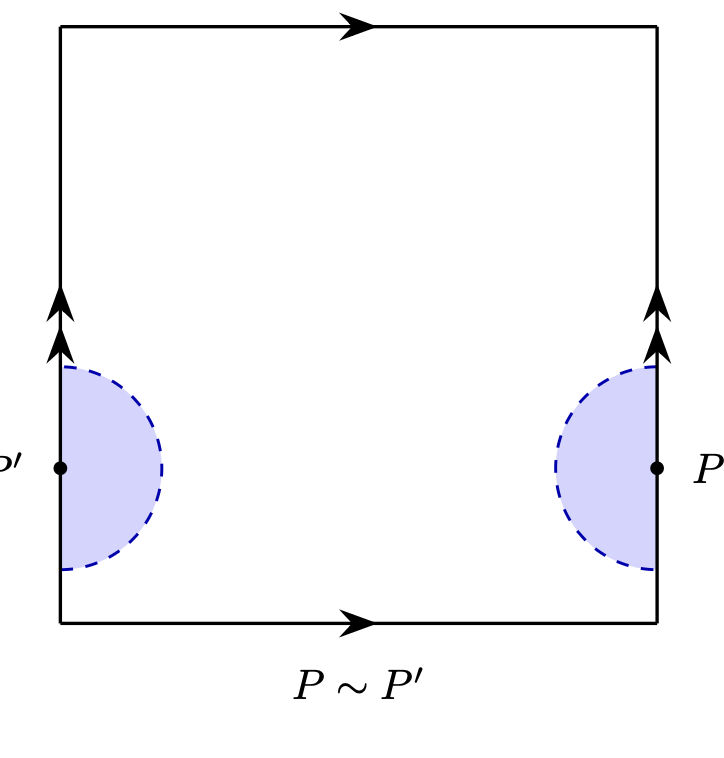
\includegraphics[width=0.5\textwidth]{Diagrams/Topology_WK_7_Q2.png}
\end{center}
\end{enumerate}

\vspace{1cm}
\noindent
Answer:\\
\\
(1) Let $D \subset Y$ be closed.  We need to demonstrate that $f^{-1}(D)$ is closed in $X$
to establish that the defined function $f: X \to Y$ is continuous.\\
\\
We proceed as follows:
\begin{align*}
    f^{-1}(D) &= f^{-1}(D) \cap X \\
 &= f^{-1}(D) \cap (C_1 \cup C_2) \\
 &= [f^{-1}(D) \cap C_1] \cup [f^{-1}(D) \cap C_2] \\
 &= [f_1^{-1}(D) \cap C_1] \cup [f_2^{-1}(D) \cap C_2] \tag{2.1}
\end{align*}
In (2.1) we use the fact that: $f_1|_{C_1 \cap C_2} = f_2|_{C_1 \cap C_2}$.\\
\\
In (2.1) we have, by assumption, that $f_i^{-1}(D)$ is closed induced by $C_i$ and so we have the union of two closed sets - which is closed in X's topological space.\\
\qed\\
\\
(2) Let us take the two functions to be:
\begin{align*}
    f_1 : [0,1] \times [0,3/2] \to [0,1]^2/ \sim \\
    f_2 : [0,1] \times [1/3,1] \to [0,1]^2/ \sim
\end{align*}
The set of overlap being: $[1/3, 2/3]$.
% ============================================================
% Exercise 3
% ============================================================
\newpage
\noindent\textbf{Exercise 3.} Which of the following topological spaces are
manifolds? Which are manifolds with boundary? Which are not manifolds at all?
You do NOT have to provide a rigorous proof, but do give a brief explanation
hinting at the reason for your answer.

\begin{enumerate}[label=\roman*),itemsep=0.5em]
  \item The closed ball $\bar{B}_{\mathbb{R}^3}(0,1)
  =\{p\in\mathbb{R}^3;\ \|p\|\leq 1\}$, with the topology induced by the
  Euclidean topology of $\mathbb{R}^3$.

  \begin{center}
    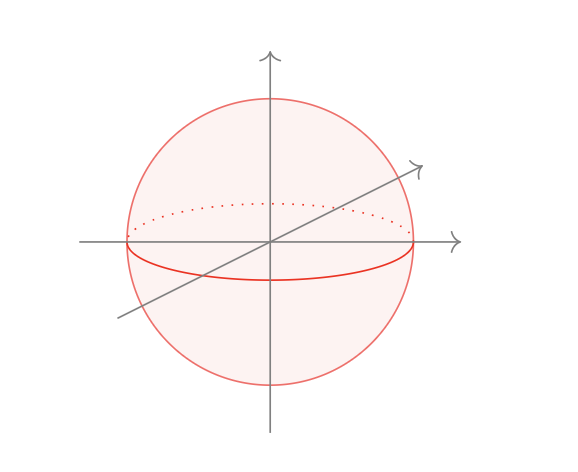
\includegraphics[width=0.5\textwidth]{Diagrams/Topology_WK_7_Q3i.png}
  \end{center}

  \item $\{(x,y)\in\mathbb{R}^2;\ x\cdot y=0\}$, with the topology induced
  by the Euclidean topology of $\mathbb{R}^2$.

  \item The closed half cone
  $\{(x,y,z)\in\mathbb{R}^3;\ x^2+y^2=z^2,\ z\leq 0\}$, with the topology
  induced by the Euclidean topology of $\mathbb{R}^3$.

  \begin{center}
    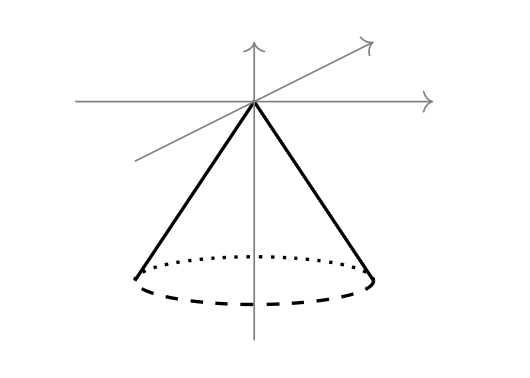
\includegraphics[width=0.5\textwidth]{Diagrams/Topology_WK_7_Q3iii.png}
  \end{center}

  \item The full cone $\{(x,y,z)\in\mathbb{R}^3;\ x^2+y^2=z^2\}$,
  with the topology induced by the Euclidean topology of $\mathbb{R}^3$.

  \begin{center}
    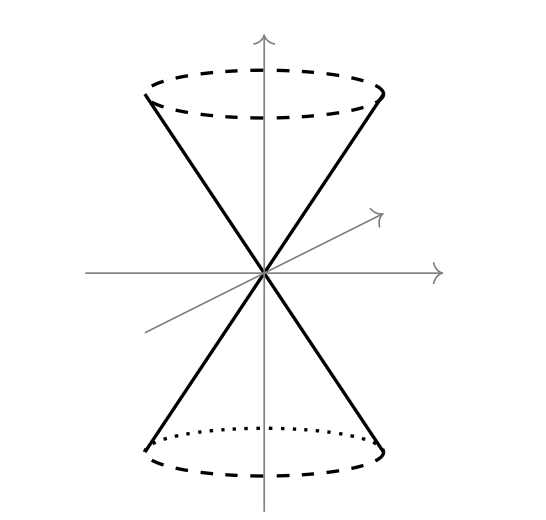
\includegraphics[width=0.5\textwidth]{Diagrams/Topology_WK_7_Q3iv.png}
  \end{center}

  \item $\mathbb{R}^2\setminus
  \{(1/n,0)\in\mathbb{R}^2;\ n\in\mathbb{N}\setminus\{0\}\}$,
  with the topology induced by the Euclidean topology of $\mathbb{R}^2$.
\end{enumerate}

\vspace{1cm}
\noindent
Answer:\\
\\
Unless specifically mentioned I will always assume that both the Hausdorff and $2^{nd}$ countable criteria
for a manifold are met.\\
\\
(i) The surface of a sphere is the the standard example of a manifold (without boundary).  We can "split" the sphere into 6 different hemispheres each
of which has a homeomorphic to an open set in $\mathbb{R}^2$.  Hence, "locally Euclidean" applies and it is a manifold.\\
\\
(ii) The set of points that satisfy the condition are the x and y axes in $\mathbb{R}^2$.\\
This is NOT a manifold.  The reson being that if one point is removed anywhere from the given set we will have a disconnected set.\\
Any single point removed from an open set in $\mathbb{R}^2$ will not create a disconnected set.  Hence, the two sets can't be homeomorphic.\\
\\
(iii)
% ============================================================
% Exercise 4
% ============================================================
\newpage
\noindent
\textbf{Exercise 4.} Let $M$ be any topological 2-dimensional manifold.
Show that the connected sum of $M$ and $S^2$ is homeomorphic to $M$ itself.

\noindent
[Hint. Use the gluing lemma and the fact that if $D\subset S^2$ is homeomorphic
 to a disk, then $S^2\setminus D$ is also homeomorphic to a disk.]

% Write your solution to Exercise 4 here.

% ============================================================
% Exercise 5
% ============================================================
\newpage
\noindent\textbf{Exercise 5.} Find a subset of the projective plane
$\mathbb{RP}^2$ that is (homeomorphic to) a M\"obius band, then show that by
removing this M\"obius band, the remaining subspace is homeomorphic to a square.
(Hint, use the following square representation of the projective plane.)

\begin{center}
    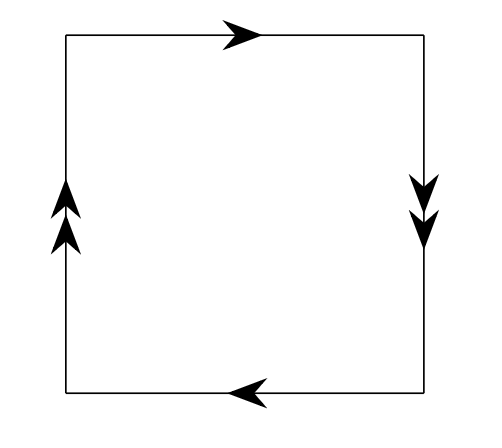
\includegraphics[width=0.5\textwidth]{Diagrams/Topology_WK_7_Q5.png}
\end{center}

% Write your solution to Exercise 5 here.

% ============================================================
% Exercise 6
% ============================================================
\newpage
\noindent\textbf{Exercise 6.} Recall that the M\"obius band $M$ is the space
obtained by gluing a square with the following identification:

\begin{center}
    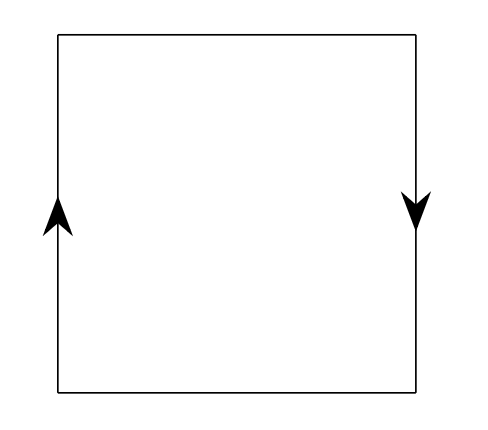
\includegraphics[width=0.5\textwidth]{Diagrams/Topology_WK_7_Q6.png}
\end{center}

\begin{enumerate}[label=\roman*)]
  \item Take a strip of paper and glue it into a M\"obius band.
  (Much easier with a long thin strip -- don't try it with a square!)
  First check that it has only $1$ face by drawing a line with a pen along
  the middle line. Now take a pair of scissors and cut it along the middle
  lengthwise (see left picture below). Observe what you get.

  \item Make another M\"obius band, but now instead of cutting in the middle,
  cut close to the edge, say at height $\frac{1}{3}$ as in the right picture below.
  (Keep cutting until you get back to where you started!)
  What do you get this time?
\end{enumerate}

\begin{center}
    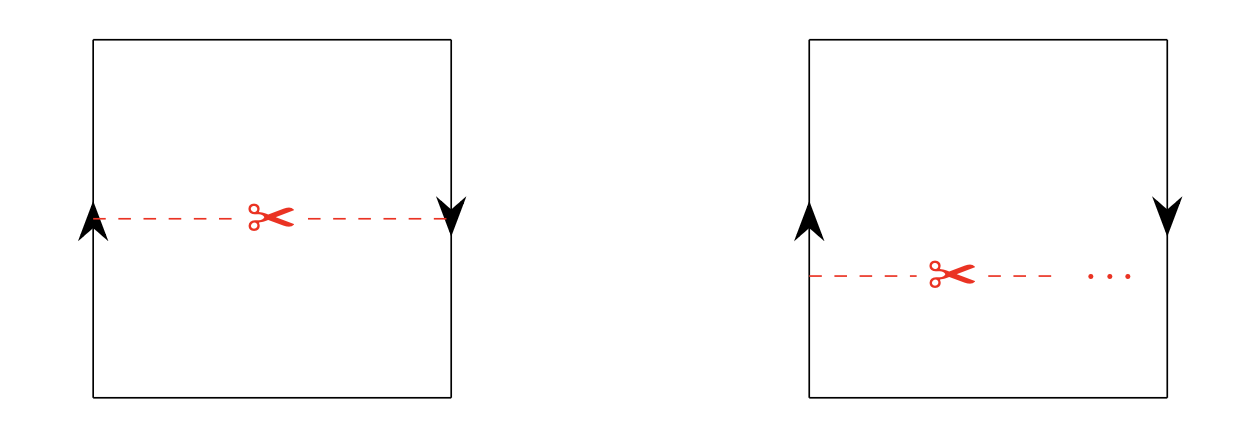
\includegraphics[width=0.5\textwidth]{Diagrams/Topology_WK_7_Q6ii.png}
\end{center}

\begin{enumerate}[label=\roman*),start=3]
  \item Think of $M$ as the square with identifications again. Let $n\geq 2$.
  If you cut it at heights $\frac{k}{n}$ for $1\leq k\leq n-1$, how many
  connected components do you get? Do they have $1$ or $2$ faces?
  What are they homeomorphic to?
\end{enumerate}

% Write your solution to Exercise 6 here.

\end{document}